\section{Operação Regenerativa sob Torque Negativo ($T_L = -T_{nom}$)}\label{sec:operacao_regenerativa}

A aplicação de um conjugado mecânico motriz externo no eixo reverte o sentido do escorregamento relativo e transporta a máquina para o quadrante operacional de gerador de indução hipersíncrono. A simulação desse regime dinâmico no Simscape SPS comprova a injeção contínua de potência ativa na rede elétrica de alimentação, vinculada à absorção ininterrupta de potência reativa para sustentação do campo girante de magnetização no entreferro.

% =========================================================================
% [DIRETRIZ DE REDAÇÃO]
% - Objetivo: Atender ao Item 2.E de sim_proj.pdf. Simular a máquina operando com torque negativo
%   (T_L = -T_nom = -20,6020 N*m), analisando o regime de gerador de indução hipersíncrono.
% - Formulação: Apresentar a teoria da conversão eletromecânica no quadrante gerador:
%   n > n_s (1885,3 rpm > 1800 rpm) \implies s < 0 (-0,0474) \implies R_2'/s < 0.
%   Demonstrar a reversão da potência ativa (P < 0, injeção na rede) e o consumo contínuo de reativo (Q > 0).
% - Figuras/Tabelas: Incluir os 3 gráficos do regime regenerativo:
%   item2e_regenerative_speed.png, item2e_regenerative_torque.png e item2e_regenerative_powers.png.
% - Confronto: Confrontar os valores numéricos simulados estabilizados (n = 1885,3 rpm,
%   T_e = -29,01 N*m, P = -2860 W, Q = +3305 var) com os fundamentos teóricos de máquinas CA.
% =========================================================================

Em $t = \SI{2,0}{\second}$, aplica-se $T_L = -\SI{20,6020}{\Nm}$, atuando o torque como máquina motriz primária. A rotação ultrapassa a velocidade síncrona ($n > n_s$), estabelecendo escorregamento estritamente negativo e resistência aparente refletida negativa:
\begin{equation}
s_{regen} = \frac{1800 - 1885{,}3}{1800} = -0{,}04739, \qquad \frac{R_2'}{s_{regen}} = \frac{\SI{1,180}{\ohm}}{-0{,}04739} = -\SI{24,90}{\ohm} < 0.
\label{eq:escorregamento_negativo_regen}
\end{equation}

\subsection{Dinâmica Hipersíncrona e Conjugado de Frenagem}\label{subsec:regen_speed_torque}

As \Cref{fig:regen_velocidade,fig:regen_torque} exibem a evolução temporal da rotação e do conjugado eletromagnético sob torque motriz.

\begin{figure}[H]
\centering
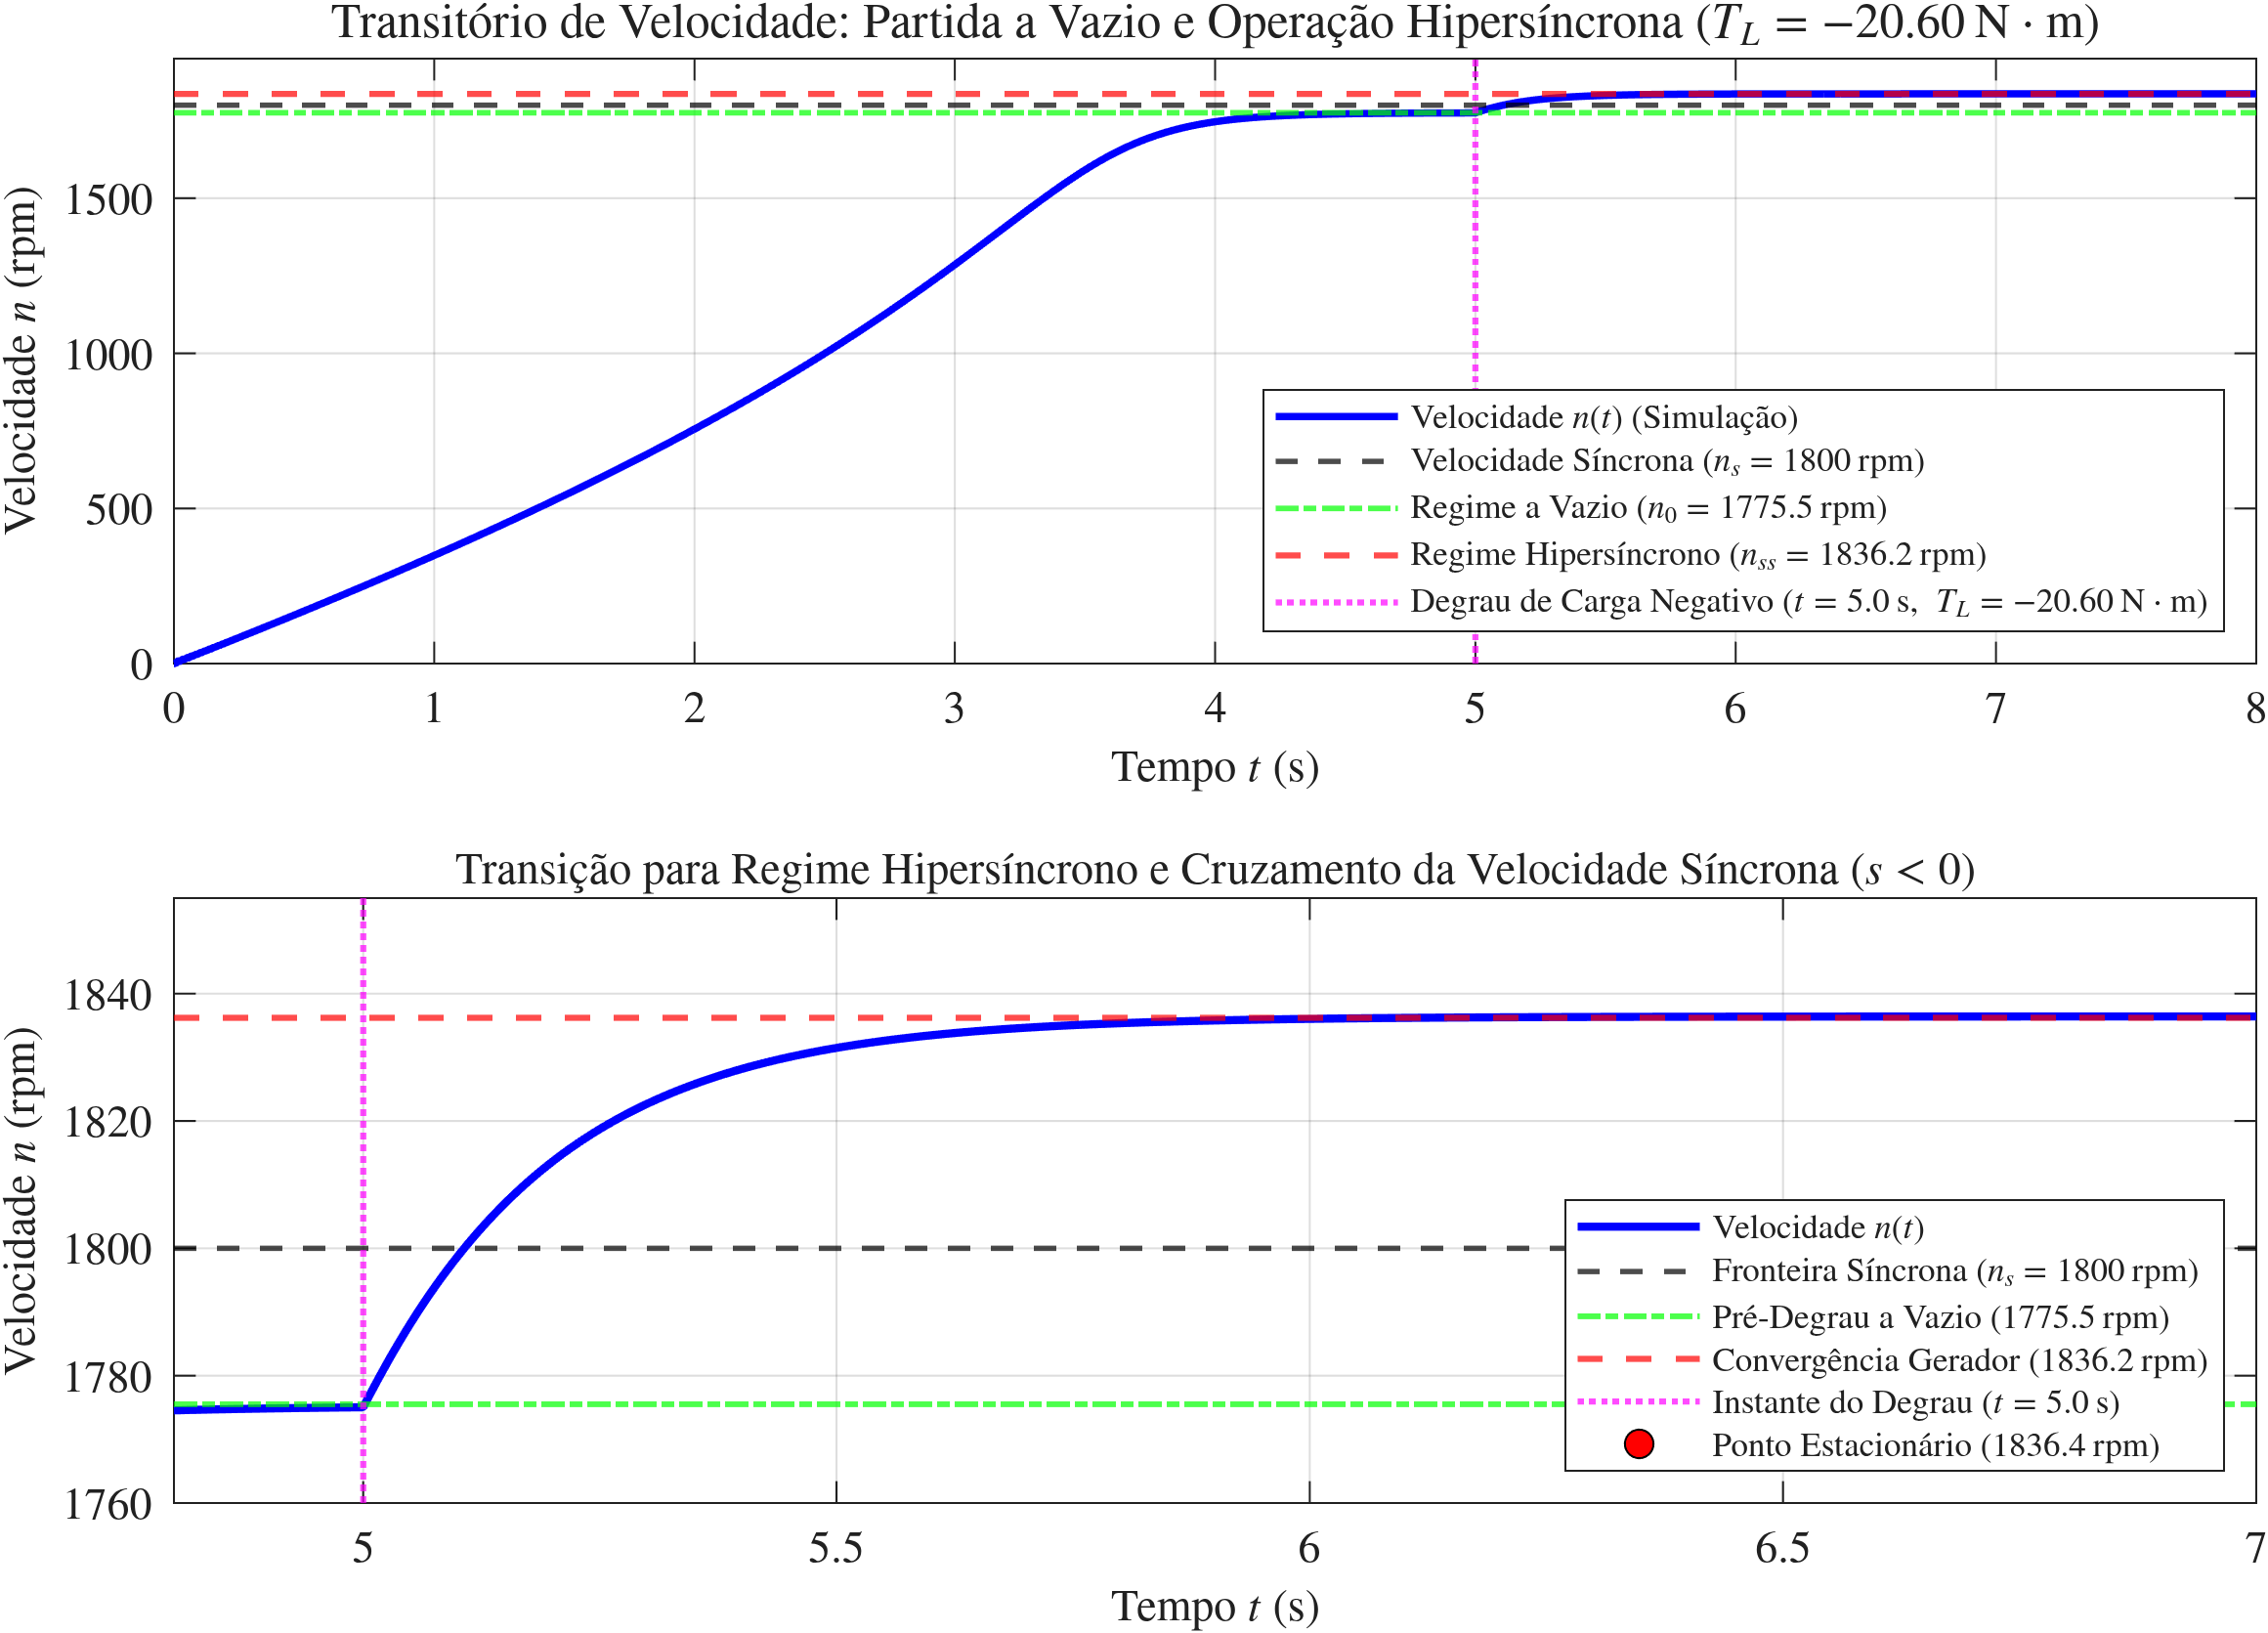
\includegraphics[width=0.82\textwidth]{item2e_regenerative_speed.png}
\caption{Resposta da Velocidade Mecânica na aceleração hipersíncrona ($T_L = -\SI{20,6020}{\Nm}$).}
\label{fig:regen_velocidade}
\end{figure}

\begin{figure}[H]
\centering
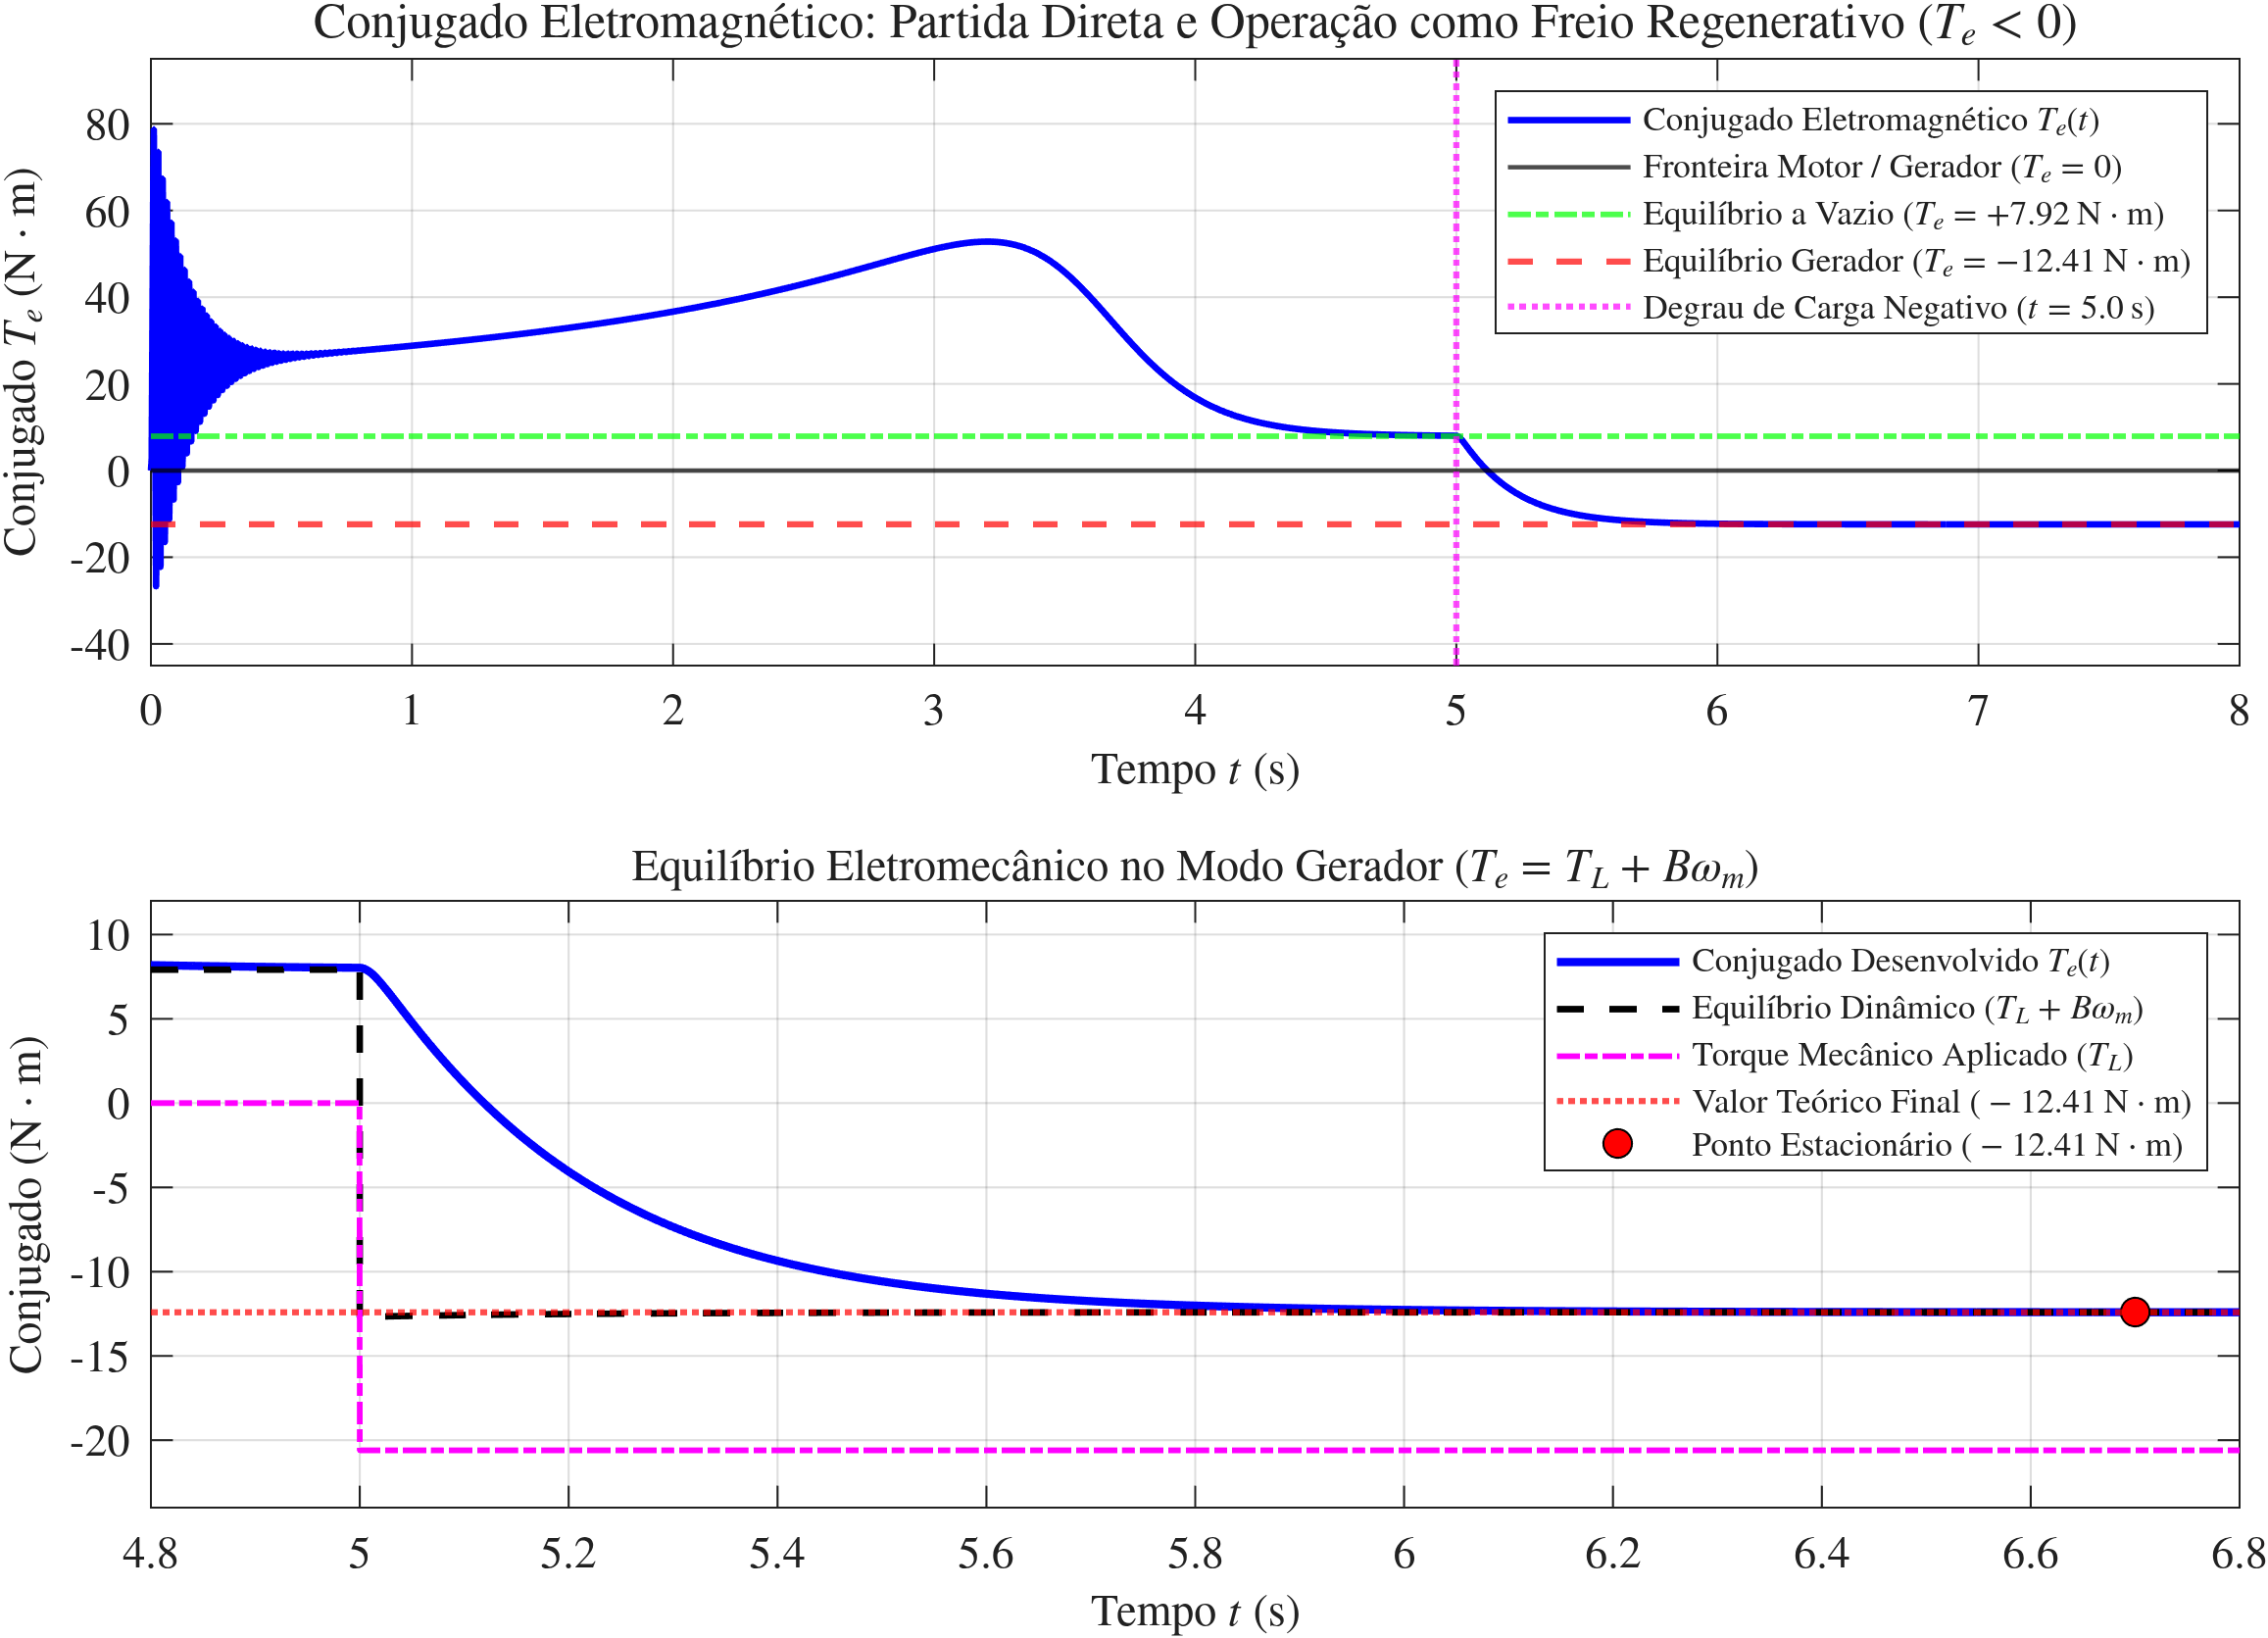
\includegraphics[width=0.82\textwidth]{item2e_regenerative_torque.png}
\caption{Conjugado Eletromagnético de frenagem desenvolvido no regime de gerador de indução.}
\label{fig:regen_torque}
\end{figure}

A rotação estabiliza em $n = \SI{1885,3}{\RPM}$ e o conjugado eletromagnético de frenagem acomoda-se em $T_{em} = -\SI{29,01}{\Nm}$, equilibrando o torque motriz aplicado e o atrito da bancada.

\subsection{Reversão do Fluxo de Potência Ativa e Demanda de Reativo}\label{subsec:regen_potencias}

A \Cref{fig:regen_potencias} ilustra a transição dos fluxos de potência nos terminais da máquina.

\begin{figure}[H]
\centering
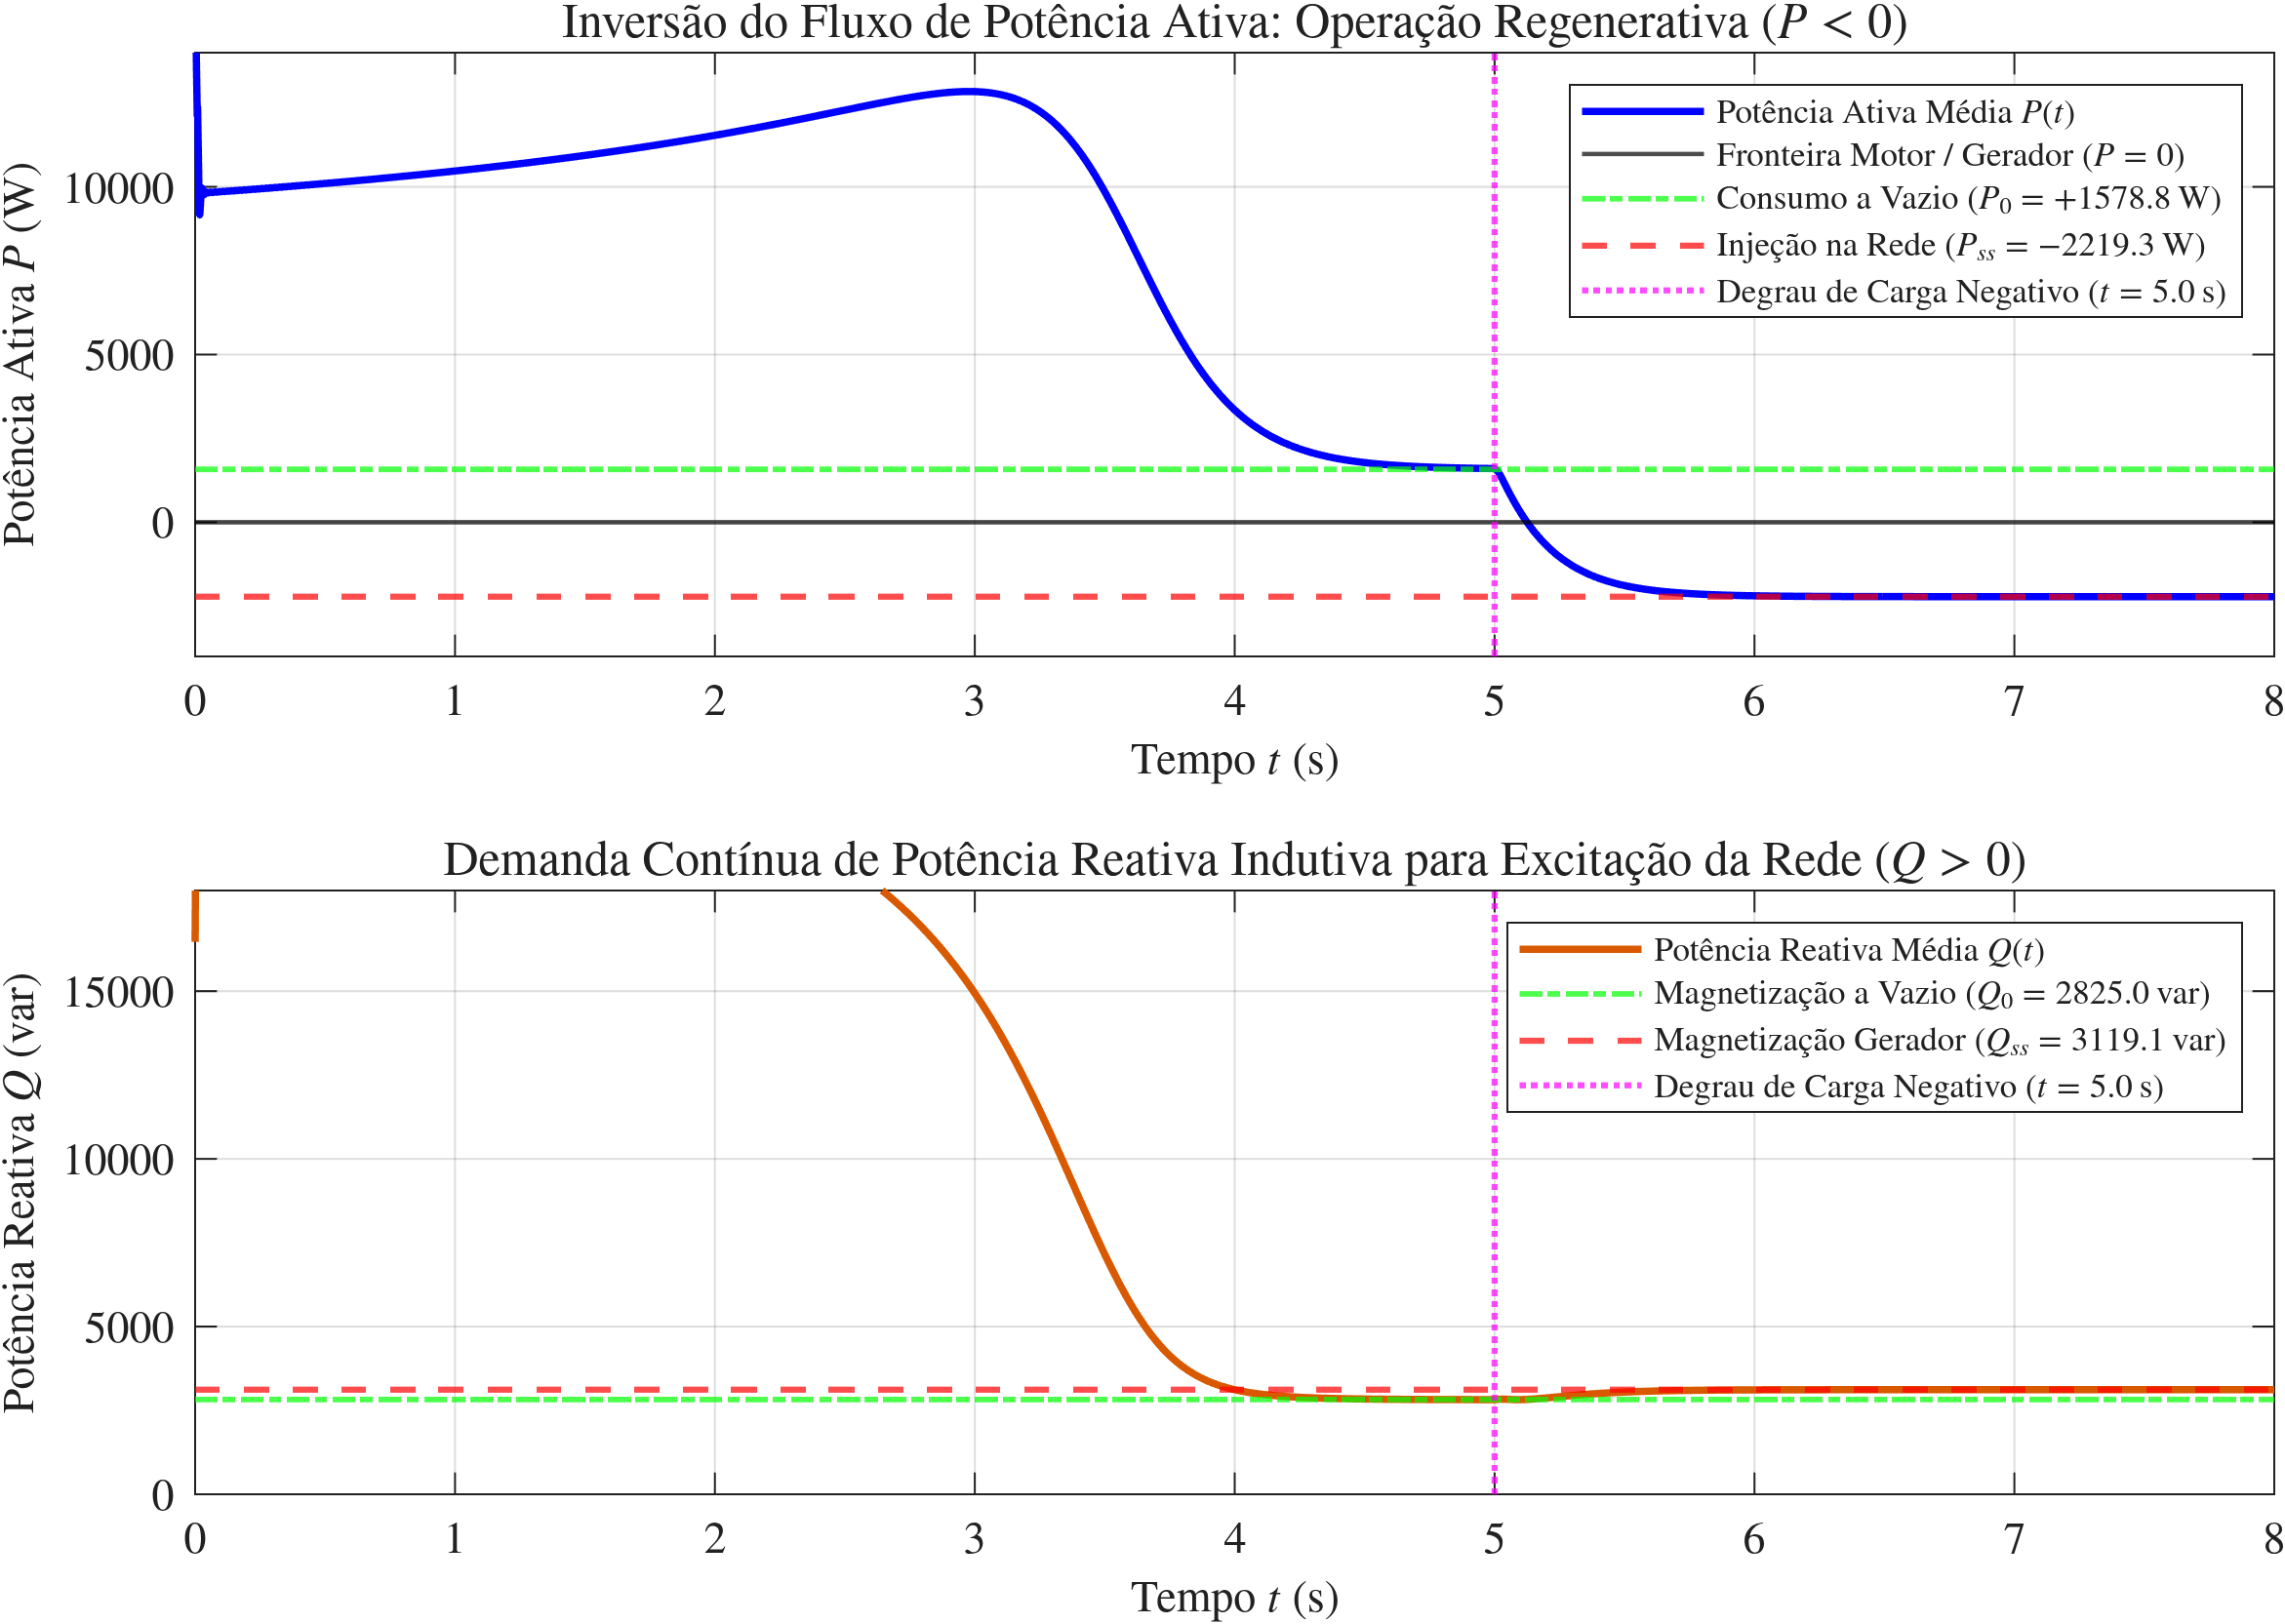
\includegraphics[width=0.82\textwidth]{item2e_regenerative_powers.png}
\caption{Dinâmica das Potências Ativa ($P$) e Reativa ($Q$) com injeção regenerativa de potência ativa na rede.}
\label{fig:regen_potencias}
\end{figure}

A potência ativa inverte o sentido de fluxo e estabiliza em $P = -\SI{2860}{\watt}$ (potência injetada na rede de \SI{220}{\volt}), enquanto a potência reativa permanece positiva ($Q = +\SI{3305}{\text{var}}$), atestando a dependência do gerador assíncrono em relação à excitação reativa da rede.
